\begin{frame}{Model for oscillating system}
From our experiment we have $(\omega_i, X_i)$ $i=1,...,N$ pairs, where $N$ is number of measurements. We can \textit{assume} that our measurements come from distribution
  \begin{equation*}\label{eq:distribution}
  X_i \, \overset{\text{iid}}{\sim} \,  
  \mathcal{P}(\,\, \cdot \,\, | \, \omega_i, \omega_0, X_0, \gamma) \equiv \mathcal{N}(X(\omega_i; \, \omega_0, X_0, \gamma),\,\sigma^{2})\ \quad 
  \text{   for   } i=1,...,n
  \end{equation*}
  \begin{equation*}\label{eq:solution-amplitude-new}
  \text{where} \ X(\omega; \, \omega_0, X_0, \gamma) = \frac{X_0 \, \omega_0^2} {\sqrt{(\omega_0^2-\omega^2)^2+(2 \gamma \omega)^2}}
  \end{equation*}
  \pause
  As precision of our measurements is 0.1, we take $\sigma = 0.1$.
  
  Our task is to estimate parameters $\omega_0,\, \gamma$ and $X_0$ from the resonance curve $(\omega_i, X_i)_{1...n}$. More formally, find \textbf{posterior distribution}
  \begin{equation}\label{eq:inference1}
  \omega_0, \, \gamma, \, X_0 \sim \mathcal{P}(\,\, \cdot \,\, | \, \omega_1...\omega_n, X_1...X_n)
  \end{equation}
\end{frame}

\begin{frame}{Using Bayes' Theorem}
For Posterior distribution we have
\begin{align*}
  \begin{split}
  \mathcal{P}(\omega_0, \gamma,X_0\,|\,X_1...X_n, \omega_1...\omega_n) &=
  \cfrac{\mathcal{P}(X_1...X_n\,|\,\omega_0,\gamma,X_0,\omega_1...\omega_n) \cdot
  	\mathcal{P}(\omega_0,\gamma,X_0)
  }{\textit{margnal}} \\
\textcolor{green}{\text{i.i.d assumption} \ }&= \cfrac{\prod\limits_{i=1}^{n}\mathcal{P}(X_i\,|\,\omega_0,\gamma,X_0, \omega_i) \cdot
	\mathcal{P}(\omega_0,\gamma,X_0)
}{\textit{margnal}}
\end{split}
\end{align*}
\pause
We take \textit{Gamma distributions} for priors of $\omega_0$, $\gamma$ and $X_0$. 

\begin{figure}
	\centering
	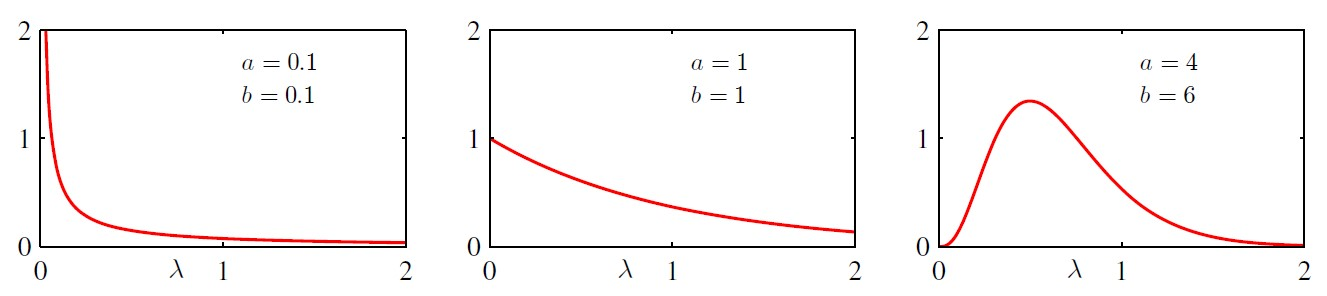
\includegraphics[width=\linewidth]{images/gamma.jpg}
	\caption{Gamma distribution pdf for different parameter values.}
\end{figure}
\end{frame}

\begin{frame}{Method}
Unfortunately we can't get analytical form of the \textit{Posterior}. But we do not need analytical form anyway. \textbf{Samples from Posterior distribution are enough!}
\\~\\
\pause
There are different sampling algorithms and frameworks. We have used \textbf{Stan}\footnotemark which uses \textit{Markov chain Monte Carlo} (MCMC) sampling algorithm.
\\~\\
\pause
Now we sample from our posterior distribution. Our samples are triplets ($\omega_0$, $\gamma$,$X_0$)\textsubscript{$i$}. \\
\textbf{Sample mean} and \textbf{sample std} for each parameter are \textbf{estimation} and \textbf{uncertainty} for that parameter respectively.

\alt<2>{\let\thefootnote\relax\footnotetext{~}}{\footnotetext{Stan statistical modeling platform \ \href{https://mc-stan.org/}{\url{https://mc-stan.org/}}}}

\end{frame}

\begin{frame}{Results}
\begin{onlyenv}<1-5>
\begin{figure}[h]
    \makebox[\textwidth][c]{%
	\includegraphics<1>[width=1.2\textwidth]{images/samples_003.png}
	\includegraphics<2>[width=1.2\textwidth]{images/samples_010.png}
	\includegraphics<3>[width=1.2\textwidth]{images/samples_030.png}
	\includegraphics<4>[width=1.2\textwidth]{images/samples_100.png}
	\includegraphics<5>[width=1.2\textwidth]{images/samples_err.png}
	}
\end{figure}
\end{onlyenv}
\end{frame}


\begin{frame}{Results}
\vspace{0.3cm}
\begin{columns}
\column{0.5\textwidth}
\Large \centering Braking current $=0.3\si{\ampere}$
\begin{figure}[t]
	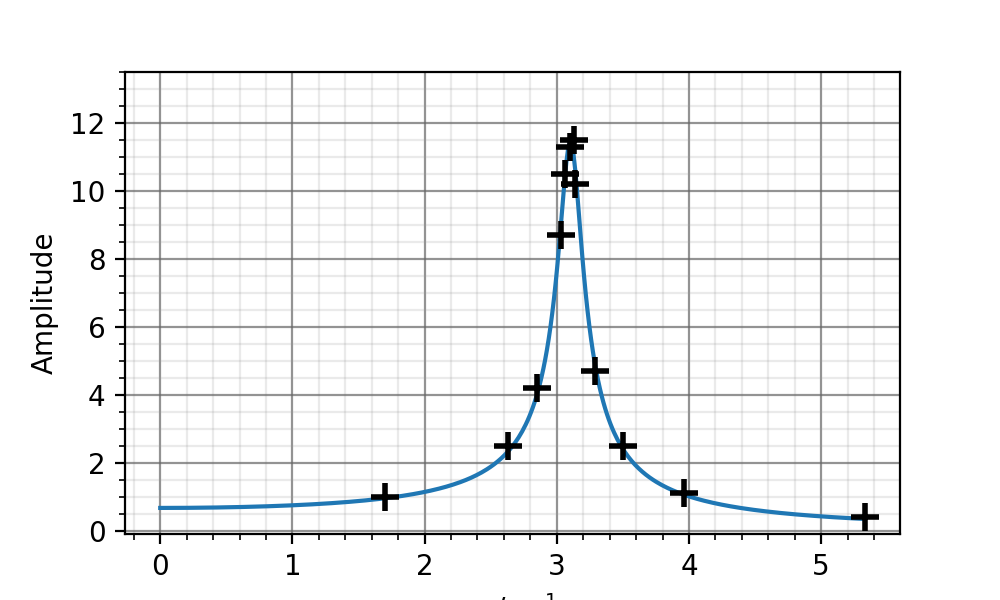
\includegraphics[width=0.95\linewidth]{images/result03.png}
\end{figure}
\column{0.5\textwidth}
\Large \centering Braking current $=0.6\si{\ampere}$
\begin{figure}[t]
	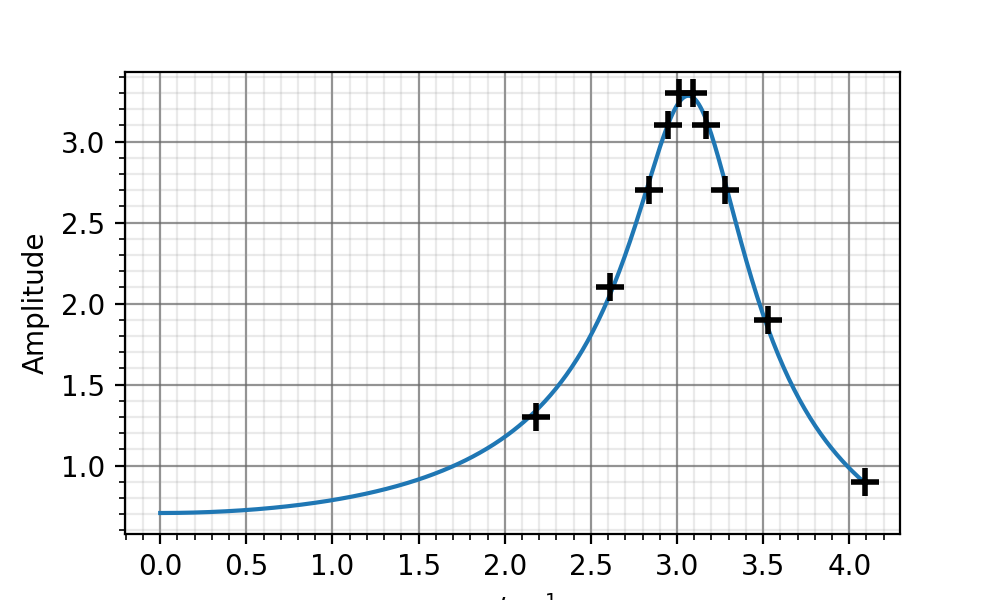
\includegraphics[width=0.95\linewidth]{images/result06.png}
\end{figure}
\end{columns}
\pause
  \begin{table}[ht]
  	\centering
  	\begin{tabular}{c c c}
  		\toprule
  		& $I_b=0.3\, \si{\ampere}$ & $I_b=0.6 \, \si{\ampere} $\\
  		\midrule
  		$\omega_0$ / \si{\per\second} & \num{3.10584 \pm 0.00012} & \num{3.1025 \pm 0.0013} \\
  		$\gamma$ / \si{\per\second} & \num{0.09059 \pm 0.00016} & \num{0.3363 \pm 0.0018} \\
  		$X_0 \equiv X(0)$ & \num{0.6675 \pm 0.0010} & \num{0.708 \pm 0.003} \\
  		$Q^{3th}$ / \si{\per\second} & \num{17.14 \pm 0.03} & \num{4.61 \pm 0.02} \\
  		\bottomrule
  	\end{tabular}
  	\caption{Resonance frequency and the amplitude at resonance.}
  	\label{table:resonance-infered-results}
  \end{table}
  
  
\end{frame}